\documentclass{beamer}
\mode<presentation> {
\usetheme{Antibes}  %Buen tema
\usecolortheme{default}
  \setbeamercovered{transparent} % Transparencia.
}
\setbeamercolor{title}{fg=white,bg=blue!90}
\setbeamercolor{block title example}{fg=white,bg=blue!90}
\setbeamercolor{block title alerted}{fg=white,bg=blue!90}
\setbeamercolor{block body alerted}{fg=blue!90,bg=white}


\usepackage[spanish]{babel}
\usepackage[utf8]{inputenc}
\usepackage[T1]{fontenc}
\usepackage{lmodern}

\AtBeginSection
{%
  \begin{frame}<beamer>
    \frametitle{Temas de la sección \thesection}
    \tableofcontents[currentsection]
  \end{frame}%
}

\title[Microprocesadores en VHDL]{Diseño de Microprocesadores en VHDL}
%\author{Ing. Eduardo José Kunysz}
%\institute[UNLP - IAR] {
%Facultad de Ingeniería (UNLP) - Instituto Argentino de Radioastronomía}
\date{26 de Mayo de 2015}


\begin{document}
\begin{frame}

\includegraphics[width=1\textwidth]{graficos/encabezado.jpg} 
%Codiseño Software Hardware
\center{Codiseño Software Hardware}
%\center{Circuitos Digitales y Microprocesadores}
\titlepage %Primer Frame para información personal.

\end{frame}
\section{VHDL y los procesadores}
\subsection{Introducción - Generalidades}
\begin{frame}
\frametitle{Introducción}
\begin{block}{VHDL}
Es un lenguaje de descripción de circuitos electrónico digitales
\end{block}
\begin{itemize}
 \item Los diseños pueden descomponerse jerárquicamente.
 \item Interconexión bién definida
 \item Se puede especificar en algoritmo o en hardware real
 \item La concurrencia, temporización y señales de reloj pueden ser todas modeladas.
 \item La operación lógica y comportamiento de temporización de un diseño pueden simularse.
\end{itemize}
\end{frame}

\subsection{Microprocesadores embebidos}
\begin{frame}
\frametitle{Hard Cores / Softcores Cores}
\textbf{Hard Cores: Silicio}
\begin{itemize}
 \item Máximas prestaciones
 \item Alto costo
 \item Dependientes del fabricante
 \begin{itemize}
  \item Xilinx Power PC $\Rightarrow$ Están migrando a ARM
  \item ARM $\Rightarrow$ Discontinuo  
 \end{itemize}
\end{itemize}
\textbf{Soft Cores: VHDL / Verilog}
\begin{itemize}
 \item Mas flexible
 \item En algunos casos independiente del fabricante
\end{itemize}
\end{frame}

\subsection{Herramienta de Simulación}
\begin{frame}
\frametitle{Modelsim}
\textbf{Modelsim SE (Versión full independiente del fabricante)}
\begin{itemize}
 \item Editor de código.
 \item Compilación.
 \item Simulaciones temporales. (Add to Wave).
 \item Realizar TestBench.
\end{itemize}

\end{frame}

\section{Módulos VHDL}
\subsection{Módulos básicos}
\begin{frame}
\frametitle{Compuertas básicas}
\begin{figure}[h]
  \centering
    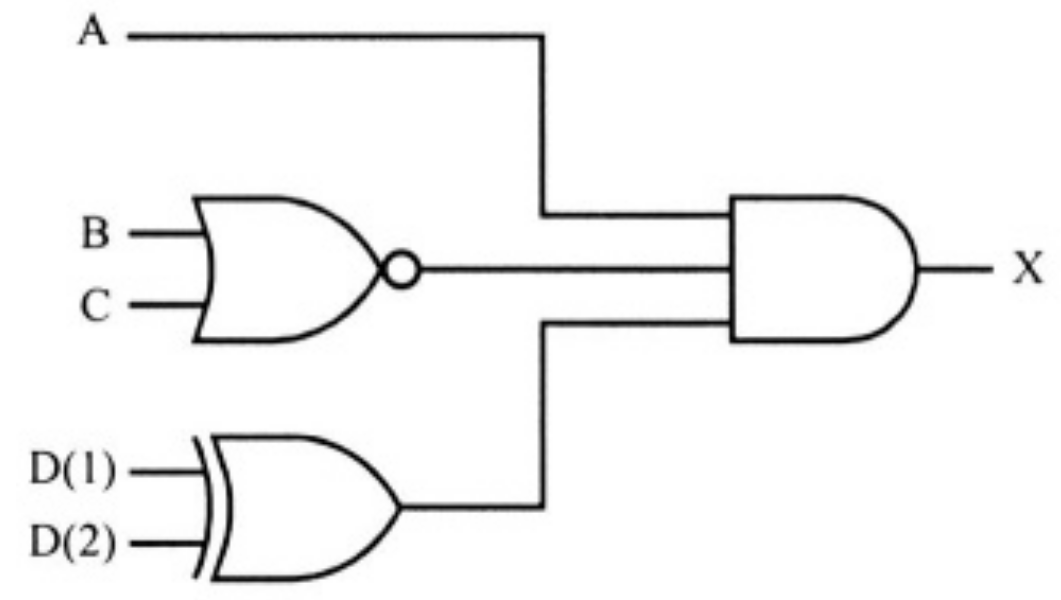
\includegraphics[width=.6\textwidth]{graficos/compuertas.png}
  \caption{Circuito digital basico basado en compuertas lógicas}
  \label{compuertas}
\end{figure}
\end{frame}

\begin{frame}
\frametitle{Flip-Flop y Registros}
\begin{itemize}
 \item El flanco positivo se selecciona mediante:

Clock’EVENT AND clock=’1’
 \item El flanco negativo se selecciona mediante:

Clock’EVENT AND clock=’0’
\end{itemize}
\begin{figure}[h!]
  \centering
    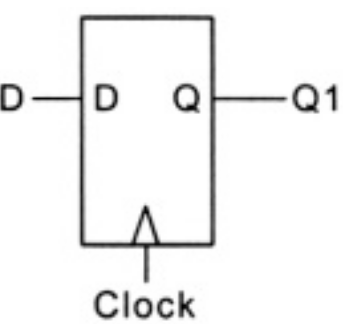
\includegraphics[width=.2\textwidth]{graficos/ff1.png}
    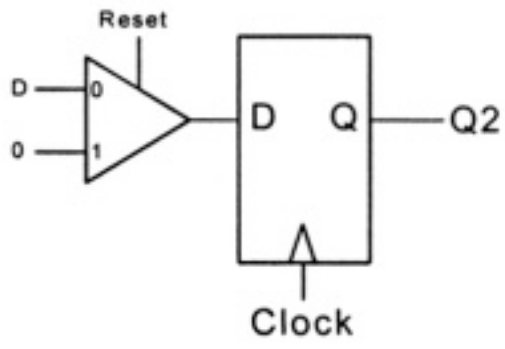
\includegraphics[width=.3\textwidth]{graficos/ff2.png}
    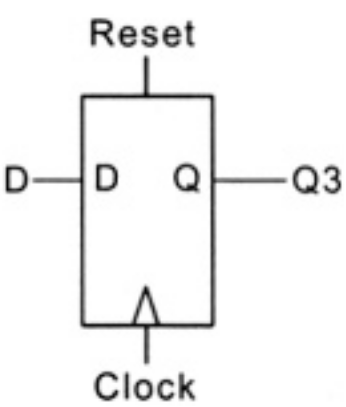
\includegraphics[width=.2\textwidth]{graficos/ff3.png}
    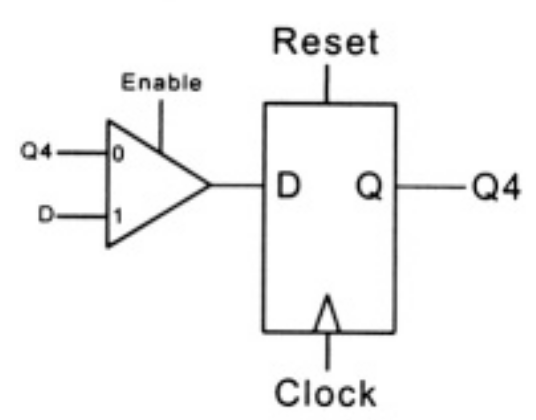
\includegraphics[width=.3\textwidth]{graficos/ff4.png}
  \caption{FF tipo D disparo por flanco positivo}
\end{figure}
\end{frame}

\begin{frame}
\frametitle{Maquinas de estado}
 \begin{figure}[h]
  \centering
    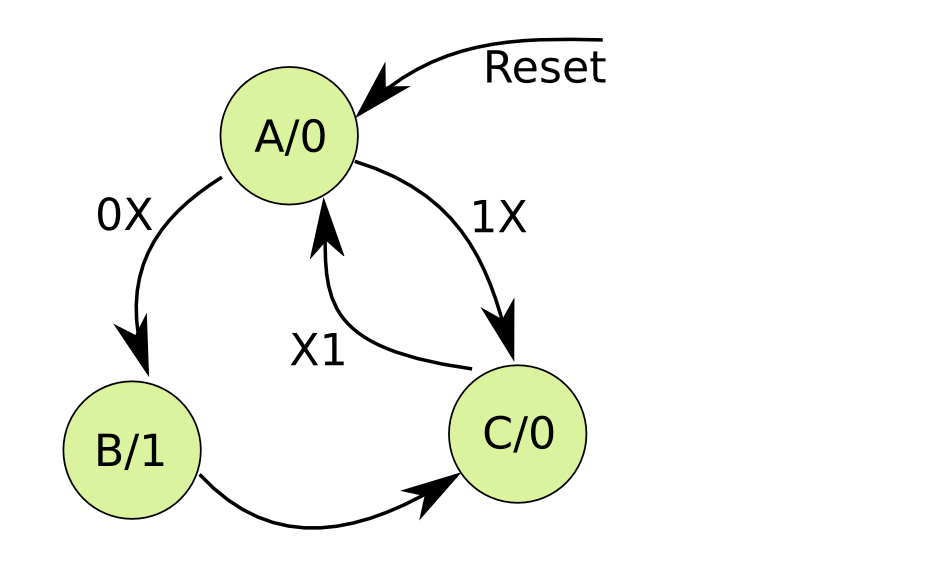
\includegraphics[width=.7\textwidth]{graficos/moore2.png}
  \caption{Máquina de estados de Moore}
\end{figure}
\end{frame}

\begin{frame}
\frametitle{Maquinas de estado}
 \begin{figure}[h]
  \centering
    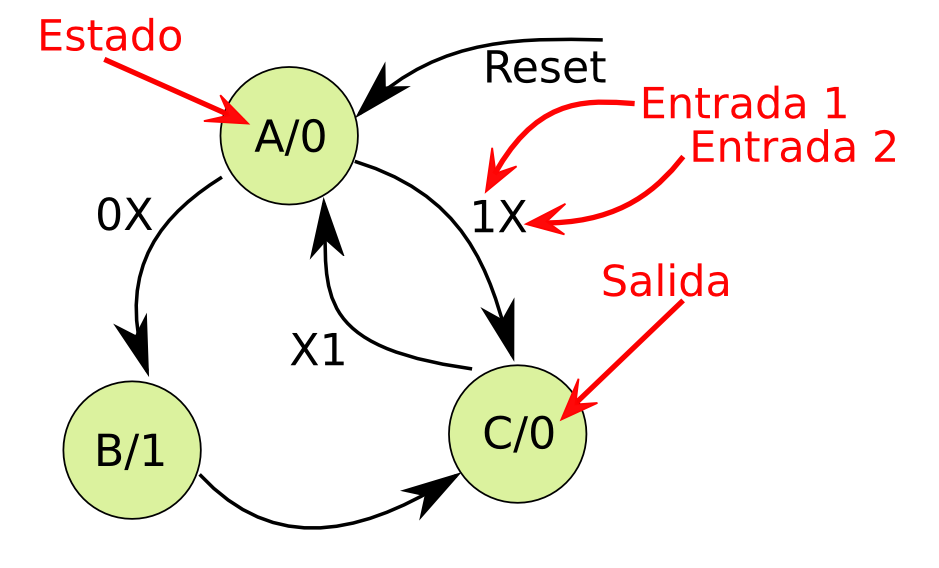
\includegraphics[width=.7\textwidth]{graficos/moore3.png}
  \caption{Máquina de estados de Moore}
\end{figure}
\end{frame}

\subsection{Modelo de una ALU}
\begin{frame}
\frametitle{ALU}
 \begin{figure}[h]
  \centering
    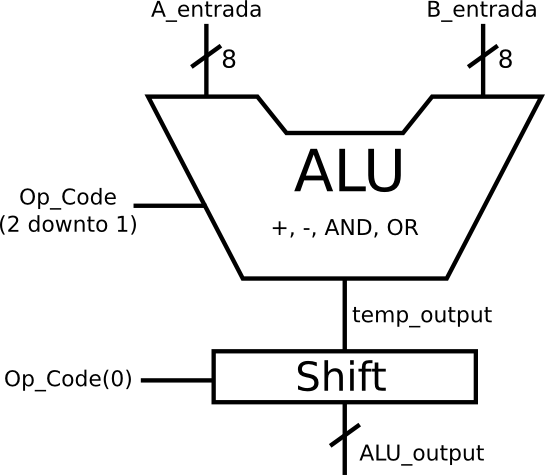
\includegraphics[width=.5\textwidth]{graficos/alu.png}
  \caption{ALU con Sumador/Restador y Desplazador}
\end{figure}

\end{frame}

\begin{frame}
\frametitle{ALU}
\begin{table}[!hbt] 
\centering
 \begin{tabular}{|c|c|}
\hline
\textbf{Op\_Codes} & \textbf{Descripción} \\ \hline
000 & Suma \\ \hline
001 & Resta \\ \hline
010 & And \\ \hline
011 & Or \\ \hline
1XX & Desplazamiento \\ \hline
\end{tabular}
  \caption{Op\_codes del módulo ALU}
\end{table}  
\end{frame}



\subsection{Modelo de una Memoria Simple}
\begin{frame}
\frametitle{Memoria} 
\begin{figure}[h]
  \centering
    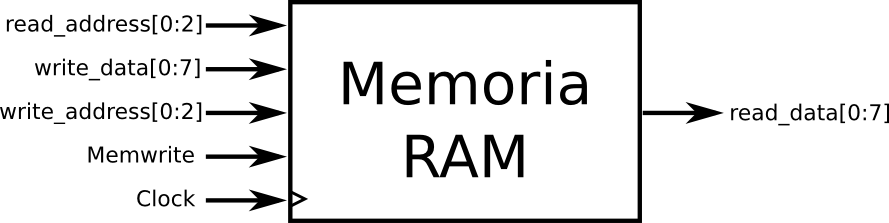
\includegraphics[width=.7\textwidth]{graficos/ram.png}
  \caption{Memoria RAM de 8 bits, capacidad 8 bytes}
\end{figure}
\end{frame}

\section{Microprocesador Sencillo}
\subsection{Arquitectura}
\begin{frame}
\frametitle{Arquitectura}  
\begin{figure}[h]
  \centering
    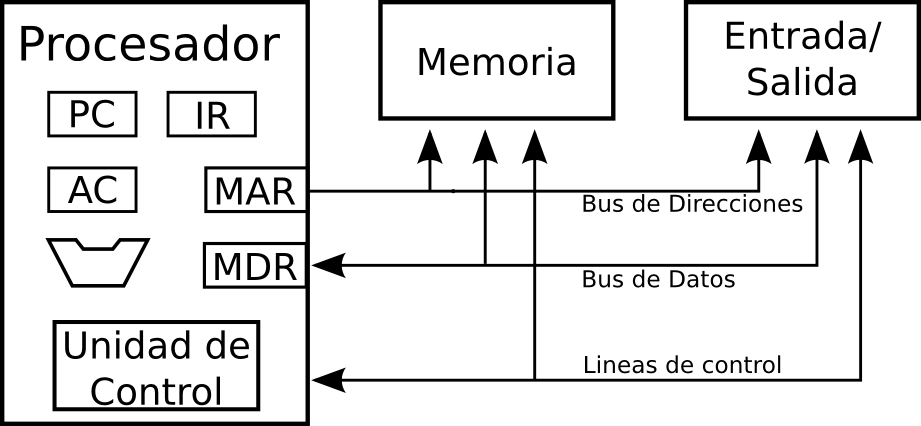
\includegraphics[width=.8\textwidth]{graficos/computadora.png}
  \caption{Arquitectura de una computadora simple}
\end{figure}
\end{frame}

\begin{frame}
\frametitle{Instrucciones}  
\begin{figure}[h]
  \centering
    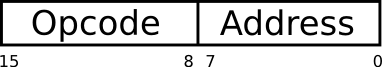
\includegraphics[width=.3\textwidth]{graficos/instruccion.png}
  \caption{Formato de la instrucción}
  \label{instruction}
\end{figure} 

\begin{table}[!hbt] 
\centering
\scriptsize{
\begin{tabular}{|l|l|c|}
\hline
 \textbf{Mnemonico} & \textbf{Operación} & \textbf{OpCode}\\ \hline
ADD dirección & AC $\Leftarrow$ AC + contenido de la dirección de memoria & 00\\ \hline
STORE dirección& contenido de la dirección de memoria $\Leftarrow$ AC & 01\\ \hline
LOAD dirección& AC $\Leftarrow$ contenido de la dirección de memoria & 02\\ \hline
JUMP dirección& PC $\Leftarrow$ dirección & 03 \\ \hline
JNEG dirección& Si AC < 0 entonces PC $\Leftarrow$ dirección & 04 \\ \hline
\end{tabular}
}
  \caption{Set de Instrucciones}
\end{table}  
\end{frame}

\subsection{Ciclos de la Instrucción}
\begin{frame}
\frametitle{Fetch, Decode, Execute}   
\begin{figure}[h]
  \centering
    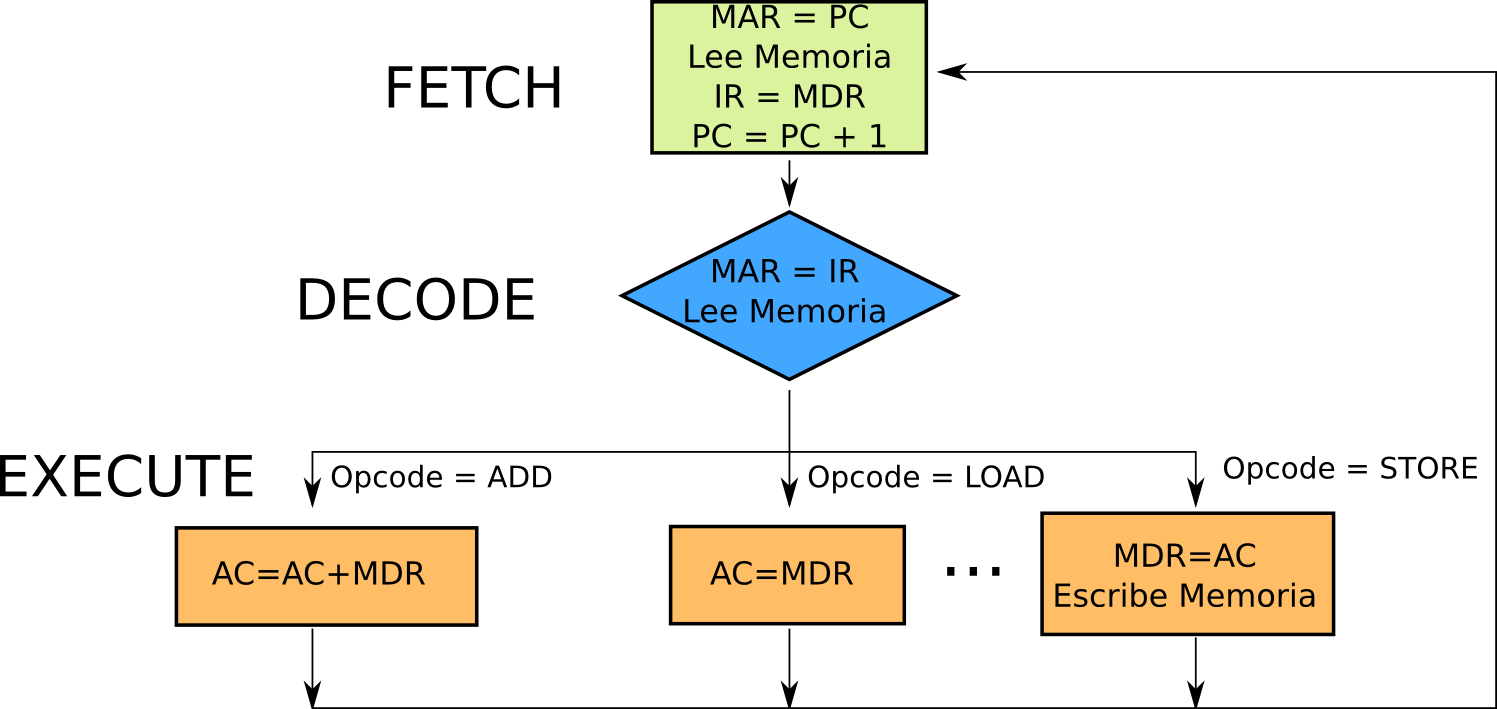
\includegraphics[width=1\textwidth]{graficos/fde.png}
  \label{instruction}
\end{figure} 
\end{frame}

\subsection{Simulación}
\begin{frame}
\frametitle{Programa a simular}   
\center {A =\$10, B =\$11, C =\$12}
\begin{table}[!hbt] 
\centering
\scriptsize{
 \begin{tabular}{|c|c|}
\hline
\textbf{Assembler} & \textbf{Código de máquina} \\ \hline
LOAD B & 0211 \\ \hline
ADD C & 0012 \\ \hline
STORE A & 0110 \\ \hline
\end{tabular}
}
\end{table}  

\begin{table}[!hbt] 
\centering
\scriptsize{
\begin{tabular}{|l|l|c|}
\hline
 \textbf{Mnemonico} & \textbf{Operación} & \textbf{OpCode}\\ \hline
ADD dirección & AC $\Leftarrow$ AC + contenido de la dirección de memoria & 00\\ \hline
STORE dirección& contenido de la dirección de memoria $\Leftarrow$ AC & 01\\ \hline
LOAD dirección& AC $\Leftarrow$ contenido de la dirección de memoria & 02\\ \hline
JUMP dirección& PC $\Leftarrow$ dirección & 03 \\ \hline
JNEG dirección& Si AC < 0 entonces PC $\Leftarrow$ dirección & 04 \\ \hline
\end{tabular}
}
\end{table}

\end{frame}

\subsection{Implementación}
  \begin{frame}
\frametitle{Método de implementación}
  \begin{figure}[h]
  \centering
    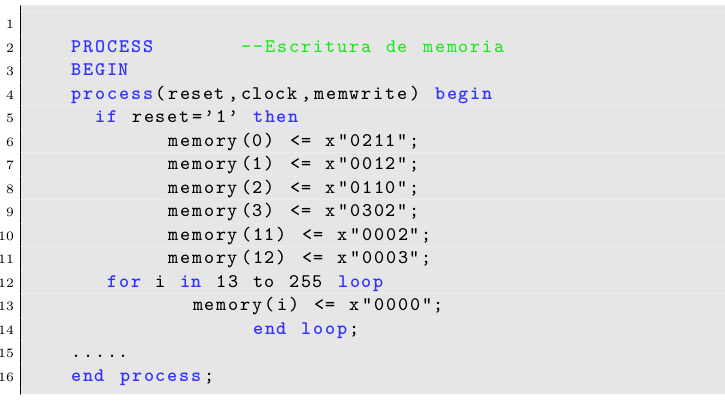
\includegraphics[width=1\textwidth]{graficos/implementacion.png}
  
\end{figure} 

  
  \end{frame}

\begin{frame}
\frametitle{Bibliografía}
\small{
[1] ``Rapid Prototyping of Digital Systems'', Sec. Edition, James O. Hamblen, M. Furmman

[2] ``Digital Design, Principles \& Practices'', Third Edition, John F. Walkerly.

[3] ``DE0 User Manual'', Altera.

[4] ``ModelSim User's Manual'', Mentor Graphics
}
\end{frame}

  
  
  \end{document}


